\chapter{Numerics}
According to \cite{erlebacher1985finite} the Gaus divergenze theorem can be rewritten as
\begin{equation}
  \label{eqn:gauss}
  \int_V \nabla \vec{F} \,\, \mathrm{d}^n V = \oint_S \vec{F} \cdot \vec{n} \,\, \mathrm{d}^{n-1}S
\end{equation}
Using $\nabla f$ for $\vec{f}$ Eqn.~(\ref{eqn:gauss}) can be rewritten as
\begin{equation}
  \int_V \nabla^2 f \,\, \mathrm{d}^n V = \oint_S (\nabla f) \cdot \vec{n} \,\, \mathrm{d}^{n-1}S
\end{equation}
For the numerical solution a cell wise desrcitization is made.
Assuming that $\nabla^2 f$ is constants over a cell the equation above reduces to
\begin{equation}
  V_C \cdot \nabla^2 f = \sum_i^N (\nabla f) \cdot \vec{n}_i \cdot A_{i}.
\end{equation}

\section{2D Application for triangular mesh}
For a trinagular mesh assuming
%----------------------------------------------------------------
\begin{figure}[ht]
    \label{fig:rod_heat_transfer}
    \centering
    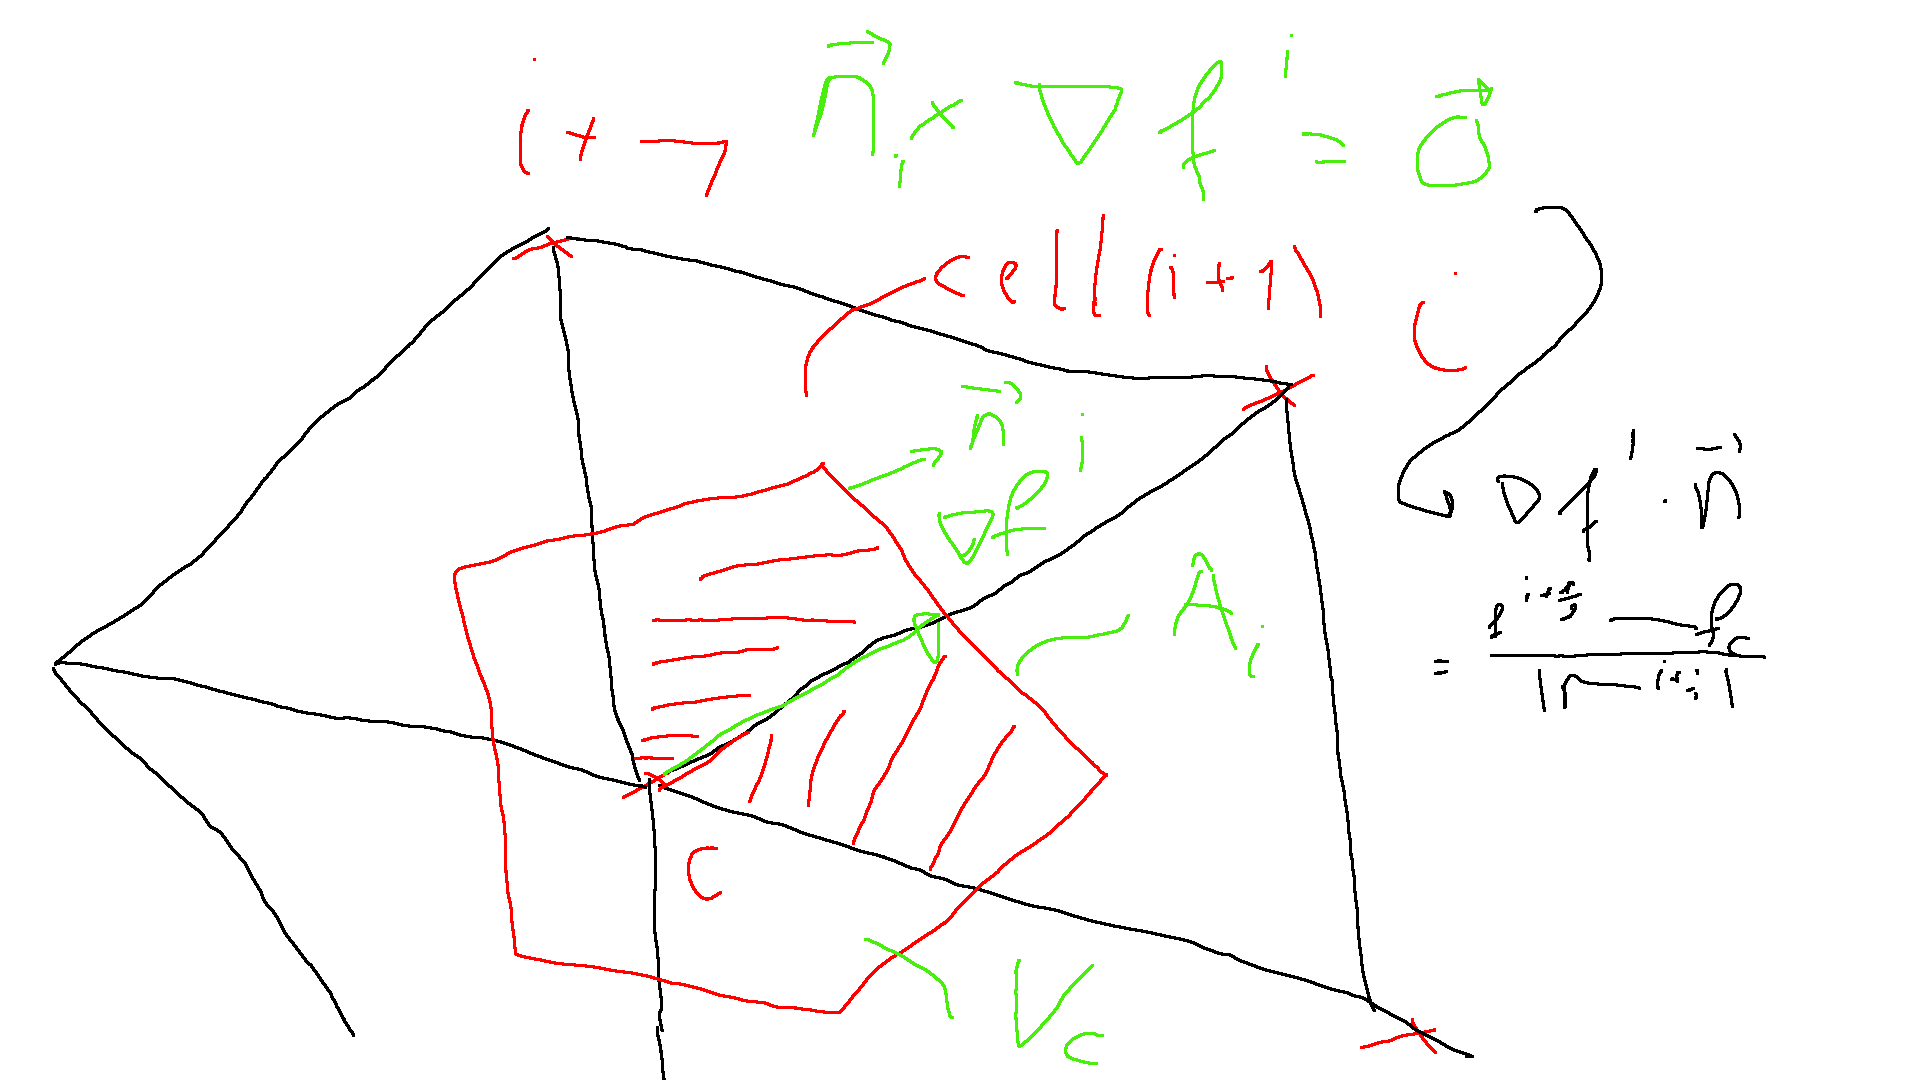
\includegraphics[width=0.8\linewidth]{draft.png}
    \caption{Test}
\end{figure}
%----------------------------------------------------------------
one can write
%----------------------------------------------------------------
\begin{equation}
  \nabla f \cdot \vec{n}_i = \frac{f_{i} - f_C}{|\vec{r}_{i}|}
\end{equation}
%----------------------------------------------------------------
for a 2d geometriy $A_{C, i}$ becomes a line segment
%----------------------------------------------------------------
\begin{equation}
  A_{i} = |\vec{b}_{i + 1} - \vec{b}_{i}| = L_i
\end{equation}
%----------------------------------------------------------------
where $\vec{b}_i$ is the barycentre of the last cell containing the point $i$.
In this context $V_C$ becomes the volume of created new cell $A_C$ which is defined as
%----------------------------------------------------------------
\begin{equation}
  A_C = \frac{1}{2} \cdot \sum_i^N  \vec{b}_{i + 1} \times \vec{b}_{i}
\end{equation}
%----------------------------------------------------------------
This leads to
%----------------------------------------------------------------
\begin{equation}
  \nabla^2 f = \frac{1}{A_C} \cdot \sum_i^N \frac{f_{i} - f_C}{|\vec{r}_{i}|} \cdot |\vec{b}_{i + 1} - \vec{b}_{i}| .
\end{equation}
%----------------------------------------------------------------
